%todo: {Accuracy of Registration} improve the perception of the MR view via accurate registration. Anatomy learning, personal information (gender, age, body shape)
\section{Personal Registration of Magic Mirror}

\subsection{Personal Information}
We augment a personalized visualization of a CT dataset onto the user. However as full CT scans of any user are generally not available, we use the Visible Korean Human dataset (VKH), which consists of a CT scan, an MR volume and a photographic volume which has been acquired by stacking up cry sections. To allow a correct augmentation of the CT data, the gender, age, body size and pose of the user has to be detected. This is performed based on the color image using the OpenBR library \cite{Klontz2013} and the depth image using the NITE skeleton tracking software. The corresponding CT volume is chosen and scaled to the size of the user and augmented onto the user body. For visualization of the bones a transfer function is used as bones can be distinguished easily in the CT volume based on their voxel intensities. For the organs a segmentation of the VKH is used. The augmentation uses contextual in-situ visualization such that the virtual objects are only shown through a circular window. This leads to a better perception of depth, compared to a simple augmentation of the whole CT. The user could naturally turn around their body to check CT volume from different viewpoints and put their right hand at different heights to select a body plane with corresponding anatomy.

\subsection{Personal Registration}
We presents a general method to interactively improve and correct the Kinect skeleton for anatomy education purposes. We believe that our general method can be applied to projectors or other sensors as well for augmented reality. A thorough validation of our method demonstrated improved precision of anatomical landmarks and opens the avenue to future improvements in medical education. Together with the ISMAR community, we hope to initiate such discussions in integrating exciting user-interaction and gaming concepts within our system.

Our AR magic mirror relies on Kinect sensor which offers an imprecise skeleton tracking output (see \figurename{\ref{fig:3-PRMM:bonelandmarker}}). This limits the precision of our magic mirror augmentations offering users false anatomical positions overlaid onto their body, resulting in a poor medical learning environment. Alternatively, had we considered projectors to display human anatomy directly on a user’s body the same inaccuracies would exist\cite{Sun2013}. 
\begin{figure}[htb]
	\centering
	\label{fig:3-PRMM:bonelandmarker}
	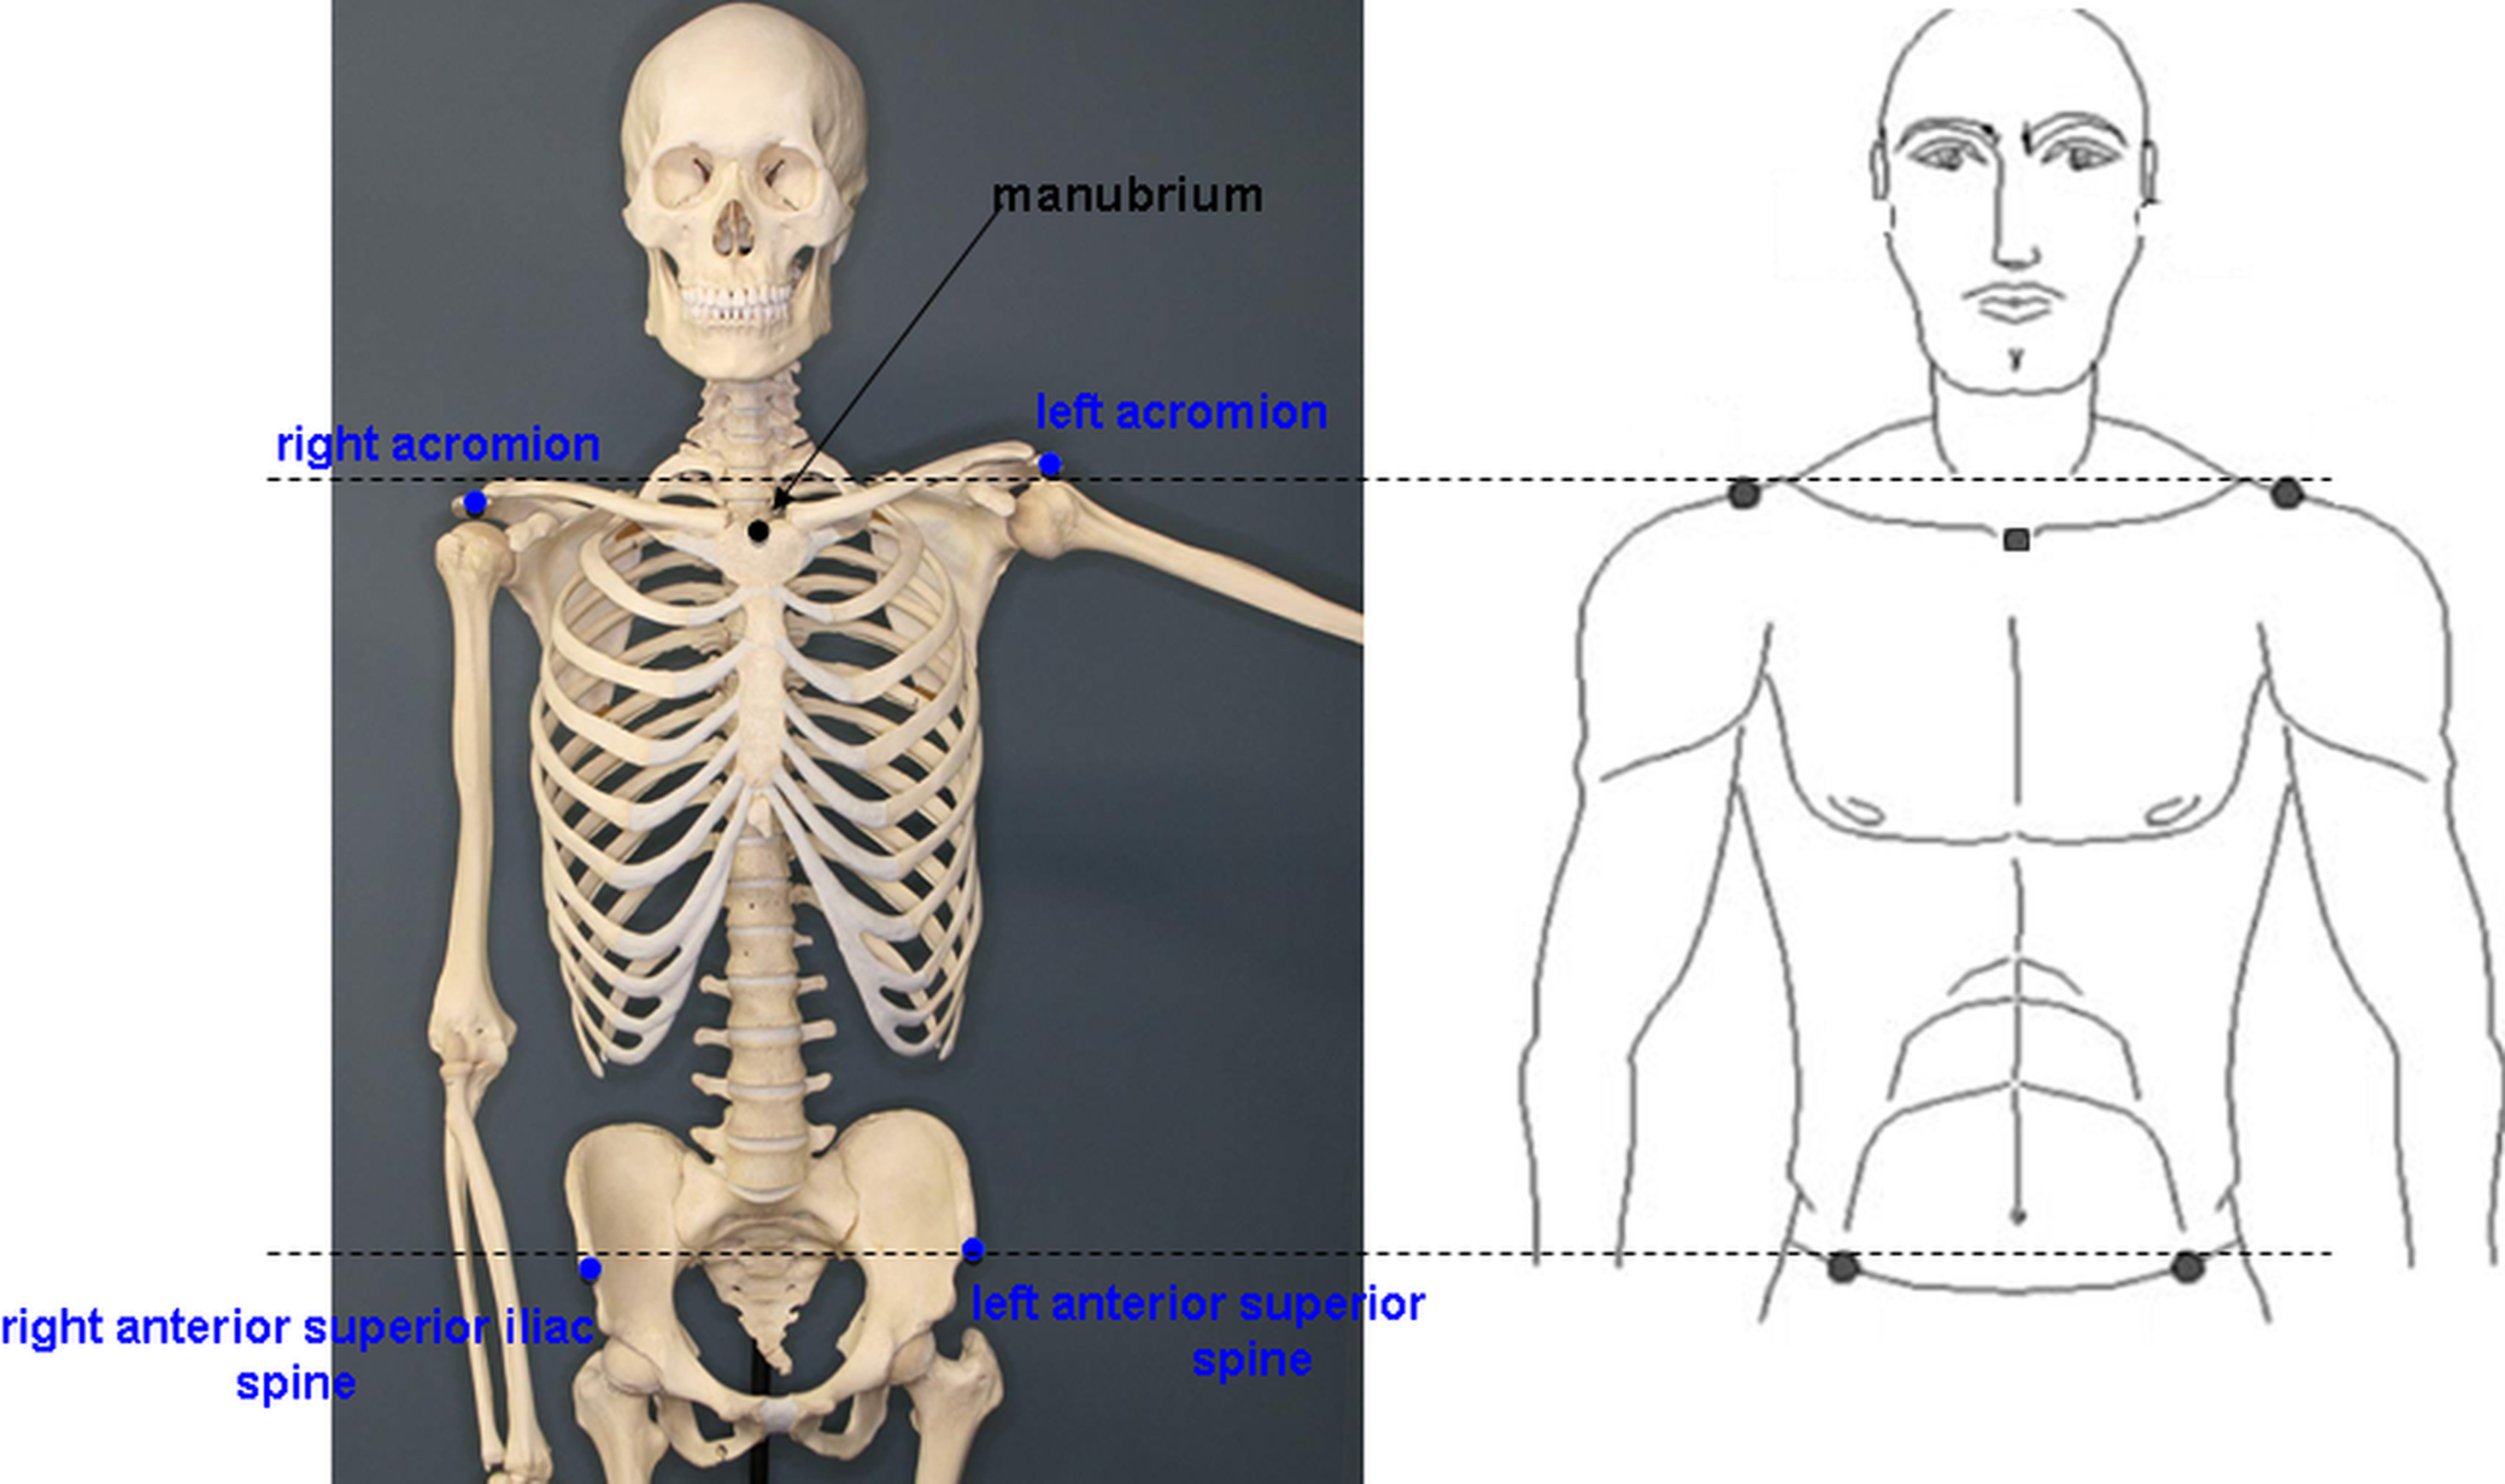
\includegraphics[width = 0.75\linewidth]{figures/3-PRMM/FiveBoneLandmarker.png}
	\caption{Selected anatomical points for Kinect skeleton improvement and subsequent CT warping and interpolation.}
\end{figure}

The goal of this method is to propose a more precise user-specific learning environment. Together with orthopedic surgeons we have defined anatomical bone landmarks: (i) which are correctly identified in medical data such as CT and (ii) which users can touch easily on their body while standing in front of any sensor. These landmark positions allow the deformation and interpolation of the medical data correctly within the magic mirror and onto the human body, resulting in a more precise Kinect skeleton and augmentation. A user study involving surgeons and anatomy experts confirm our findings. 

The skeleton output from Kinect limits the precision of the AR magic mirror applications. Thus, our magic mirror augmentations would contain errors and users would easily distinguish anatomical offsets on their body resulting in a poor anatomy learning environment. Alternatively, we had considered projectors to display human anatomy and along with their existing limitations the same inaccuracies would exist. Our aim was then to propose a method to correct for such overlay inaccuracies that could be translated to any magic mirror system worldwide. Together with orthopedic surgeons, we have defined five bone landmarks that (i) users can easily identify and touch while standing in front of the Kinect, and (ii) that are accurately and easily identified in medical data such as CT \cite{ma2013ismar}. These are: left and right acromion, left and right anterior superior iliac spine, and the manubrium (see \figurename{\ref{fig:3-PRMM:5points}}).


\begin{figure}
	\centering
	\subfloat[~Improvement of Kinect skeleton]{
		\includegraphics[height = 7cm]{figures/3-PRMM/ModifiedSkeleton.png}
		}
	\quad
	\subfloat[~Bone landmarker in CT volume]{
		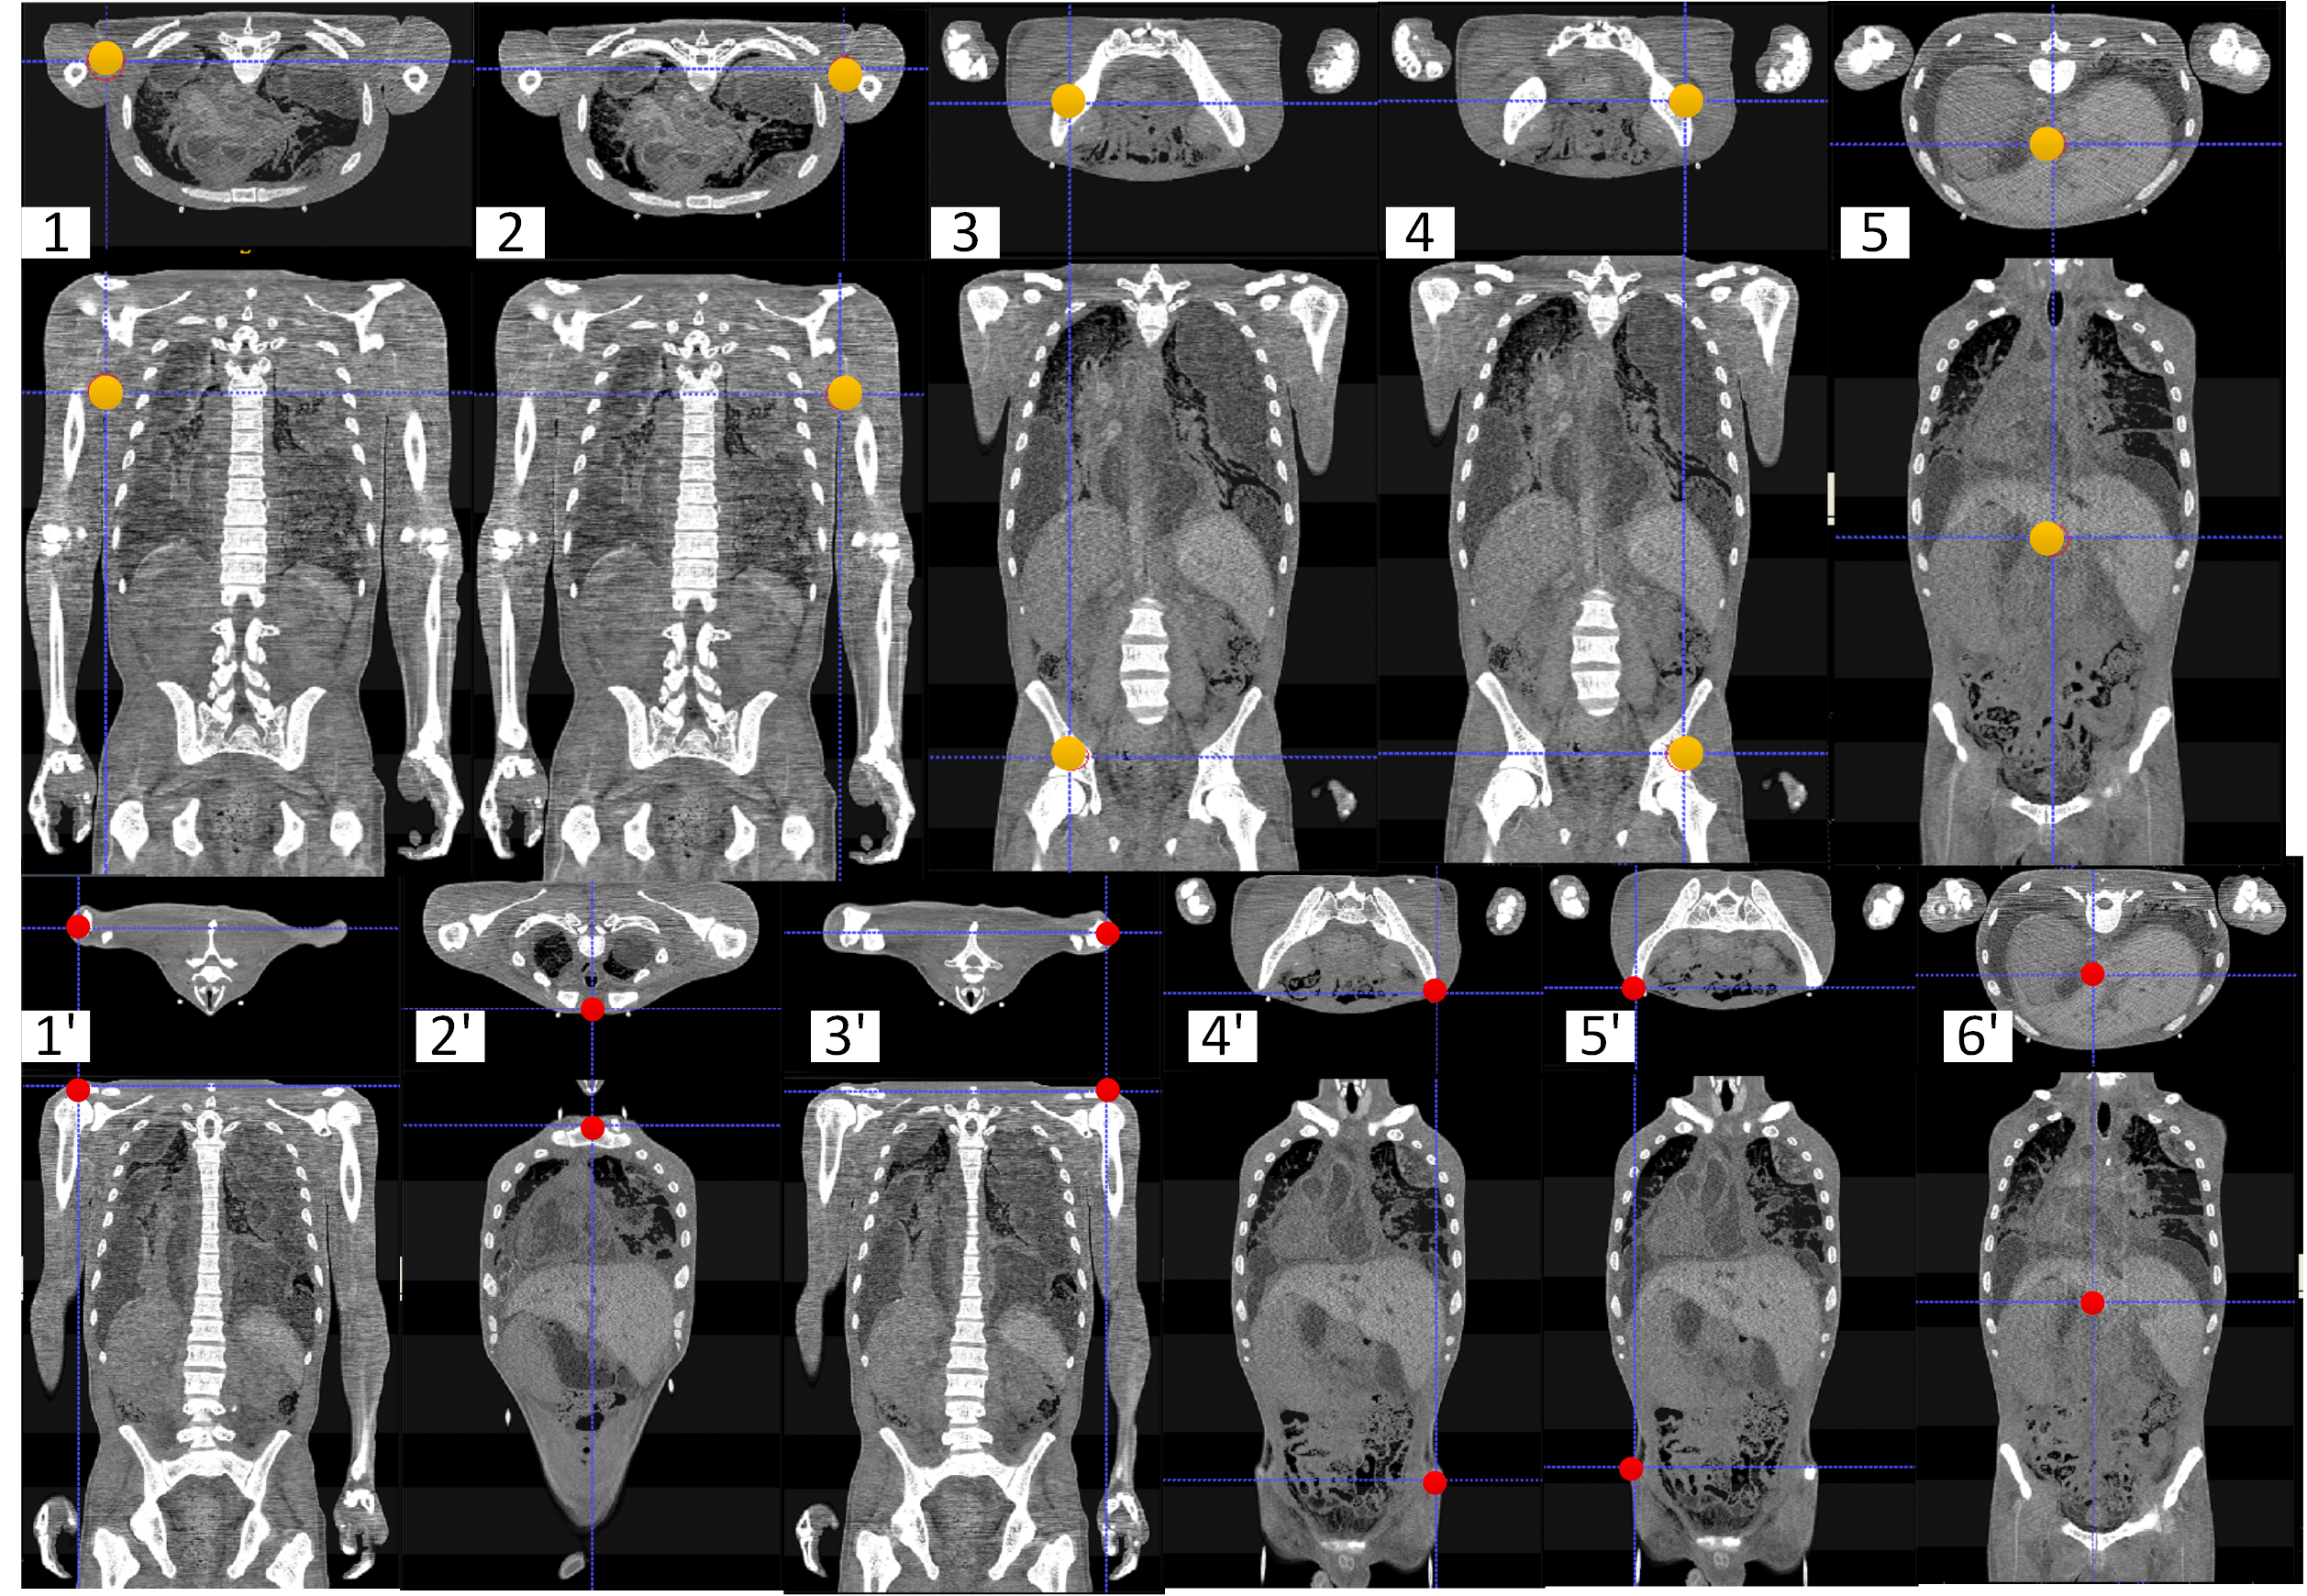
\includegraphics[height = 7cm]{figures/3-PRMM/BoneLandmarkerInCT.png}
			}
	\label{fig:3-PRMM:5points}
	\caption{(a-b) The inaccurate Kinect skeleton, in yellow, compared to the improved Kinect skeleton positions in red. (c) CT data from the Visible Human Korean showing the 5 landmarks from Kinect skeleton. (d) CT data showing correctly the 5 landmarks + interpolated torso landmark using our method.}
\end{figure} 
\subsubsection{Anatomical bone landmarkers}
Together with orthopedic surgeons, we have defined five bone landmarks that can easily be touched on the human body. These are: left and right acromion, left and right anterior superior iliac spine, and the manubrium. Subjects are positioned in front of the Kinect sensor and asked to interactively adjust the positions of five landmarks
\subsubsection{Improment of kinect skeleton}
Figure 3 shows a comparison between the traditional Kinect skeleton and its proposed improvement. The first row depicts visually the exactness of the new skeleton. The second row depicts the skeleton landmarks directly on CT data. We observe that the shoulder and anterior superior spine are inaccurate in the images. The last row depicts the improved landmark positions within CT as well. Transverse and sagittal CT slices of the visible human Korean are seen respectively in rows 2 and 3.
In Figure 3a, the following scale factors were computed for the magic mirror augmentation:

\subsubsection{Evaluation}
As an augmented reality anatomy learning application, both accuracy and system usability are very important prior to its translation in classroom. Firstly, we undertook one user study with particular users having expert anatomy knowledge to evaluate if this system is precise enough for anatomy learning. Secondly, another user study involving first year medical students took place to verify the learning potential and acceptability of our technology as a compliment to atlas textbooks in classroom.

\paragraph{Assessing the magic mirror system precision and usability}
Participants: Seven participants were included in this study (two surgeons and five final year undergraduate medical students). 
Analysis: a Likert scale was used which is a type of psychometric response scale often used in surveys and the most widely used scale in survey research. When responding to a Likert questionnaire item, respondents specify their level of agreement to a statement. The format of our 5-pt Likert was: (1) strongly disagree, (2) disagree, (3) neither agree nor disagree, (4) agree, (5) strongly agree. 
To assess the precision of our personalized magic mirror we asked the participants to interact with the system platform which integrates user-specific anatomical landmark selection. Participants were asked to provide an estimated numerical offset, if any, on how far specific bone landmarks or organs were with respect to their own body. For this, they interacted with the magic mirror window, CT data, and used their own medical knowledge and expertise for judgment. CT data was displayed in an interface depicting both transverse and sagittal planes, and participants would quantify the offsets. If needed, a ruler was provided to assist them. The anatomical targets during evaluation were defined as: the anterior superior iliac spine, manubrium, heart, and liver. Results from this exercise are shown in \tablename{\ref{tb:3-PRMM:results1}}, with offsets measured in centimeters. Results from the user study show that the precision of user-specific learning environment is on average 0.96cm.
\begin{table}
	\caption{Precision (in cm) of magic mirror system based on anatomical offsets}
	\label{tb:3-PRMM:results1}
	\scriptsize
	\begin{center}
		\begin{tabular}{p{4cm}|p{3cm}}
			Anatomy & Offset(Mean$\pm$ STDev) \\
			\hline
			anterior superior iliac spine & $0.67\pm0.52$\\
			manubrium & $0.67\pm0.75$ \\
			heart & $1.17\pm1.60$\\
			liver & $1.33\pm1.21$
		\end{tabular}
	\end{center}
\end{table}

The seven participants were then asked to judge the usability of the AR magic mirror system by responding to the following questions: (i) is the overlay accurate w.r.t human body (ii) is the user interface easy to use, (iii) is it fun to play, (iv) can it be used for medical education, and (v) would it have stronger impact for medical education learning?
The Likert scale results for the first four questions are shown in \tablename{tb:3-PRMM:results2}.
\begin{table}
	\caption{Likert scale results regarding magic mirror usability}
	\label{tb:3-PRMM:results2}
	\scriptsize
	\begin{center}
		\begin{tabular}{p{6cm}|p{3cm}}
			\space & Mean$\pm$ STDev \\
			\hline
			is the augmented reality overlay accurate w.r.t human body & $4.00\pm0.89$\\
			is the user interface easy to use & $3.67\pm1.03$ \\
			is it fun to play & $4.50\pm0.55$\\
			can it be used for medical education & $4.17\pm0.75$
		\end{tabular}
	\end{center}
\end{table}
For the last question regarding the impact of our technology, there was a unanimous response that the AR magic mirror system should be considered as a potential platform to complement existing anatomy learning tools inside anatomy classrooms. 
\subsubsection{Discussion}
The precision of our method is visually demonstrated in Figure 3c-d and \figurename{\ref{fig:3-PRMM:ResComparing}}. We observe that the acromion and anterior superior iliac spine, using the traditional Kinect skeleton, is not positioned correctly within the CT data compared to the modified Kinect skeleton version (1-2 vs. 1'-2'; 3-4 vs. 3'-4'). The orthopedic surgeons participating in our study confirmed this.
\begin{figure}
	\centering
	\includegraphics[width = \linewidth]{figures/3-PRMM/ResComparing.png}
	\label{fig:3-PRMM:ResComparing}
	\caption{Figure 4:	The magic mirror before (top) and after (bottom) the Kinect skeleton adjustment. Column 2 depicts the bottom of the rib cage being positioned correctly after skeleton correction.}
\end{figure}
Results from a user study show the impact of interactively improving the Kinect skeleton to increase precision for a better visualization of anatomy. The offsets of specific anatomical landmarks decreased significantly. The following comments were collected:
\begin{enumerate}
	\item the precision improved; making the user touch anatomical landmarks is cool since this is the way it is done in clinic…
	\item two additional landmarks easily accessible are the sternum and bottom of rib cage…
	\item make the magic mirror circle bigger for larger anatomy…
	\item voice command is a good idea but it is sensitive to the surroundings voice
	\item interactions between observers …
	\item could introduce the female CT visible human Korean…
	\item could use a healthy patient CT or other modality…
	\item could make the CT slices bigger on the screen…
\end{enumerate}

One appealing feature of the system is that with the Kinect we are using inexpensive standard hardware. In the future such a system could be made available to students or patients who have to do rehabilitation exercises at home. In addition to the full system using a large screen and a screen stand we also want to evaluate the benefit of making the system accessible to students when they are at home and at any time. We want to do this for two different reasons. First, there is a trend toward competency-based education in medicine. Instead of defining a curriculum, learning outcomes are defined. Students have to fulfill these learning outcomes. The advantage of competency-based education is that all students will have the same competency in the end. A student who is less skilled has to take more time to learn than a student who already has good skills. One requirement for this is that the students have to be able to educate themselves until they reach the required competency. We plan to use the AR magic mirror system both to allow them to do training and to test whether a learning outcome has been met. The magic mirror has to be made easily available to them so that they can use it for training at any time. The second reason to develop a distributed system which can easily be used by students is to collect user statistics.

Many medical education systems are web-based and allow accessing them from every computer. However current systems do not use high-end visualization and input devices like the Kinect. In the future when technologies like HTML5 and WebGL have matured it can be imagined that a system like the magic mirror could be implemented using web technology such that it can run on any computer. However, at the moment the use of web technology would be a significant limitation. We are using very large datasets, high-end visualization, GPU computing and gesture-based interaction.

It was originally suggested to us that our system would have much more of an impact for medical education learning if it were to be translated today in medical schools and anatomy classrooms. As such, with the help of our co-author and anatomy professor, we deliver the improved AR magic mirror to two anatomy classes within the Anatomy Department of the Ludwig Maximilian University (LMU) Medical School, Munich, Germany. The anatomy professors made it clear that the AR magic mirror system is exciting, but has to go beyond state-of-the-art technology to be truly useful for education. Our participants stressed the importance of visualization of anatomy that can change dynamically resulting from the actions of the user moving the body, and also for visualization of muscles. Furthermore, more advanced user interactions like the use of gaming elements would be required to make the use of the system for learning tasks more interesting.